\documentclass[12pt,oneside,letterpaper]{article}
\usepackage{longtable}
\usepackage{graphicx}
%\usepackage{fullpage}

\newenvironment{packed_enumerate}{ %custom enumerate for single-spacing
\vspace{-7mm}
\begin{enumerate}
  \setlength{\itemsep}{0pt}
  \setlength{\parskip}{0pt}
  \setlength{\parsep}{0pt}
}{\end{enumerate}
\vspace{-8mm}}

\pagestyle{headings}
\oddsidemargin 0.25in \textwidth     6.25in \topmargin     0.4in
\textheight    8.5in

\begin{document}


\title{\bfseries Data Classifier: \\
Software Requirements Specification\\
version 1.0}

\author {
\large{Team Mark}\\
\emph{Computer Science Department}\\
\emph{California Polytechnic State University}\\
\emph{San Luis Obispo, CA USA}\\
}

\date{October 10, 2018}
\maketitle \thispagestyle{empty}


\pagebreak
\tableofcontents

\addcontentsline{toc}{section}{Revision History}

\addcontentsline{toc}{section}{Credits}

\section*{Credits}
\begin{tabular}{|l|l|p{2.5in}|l|}
\hline
\textbf{Name}&\textbf{Date}&\textbf{Role}&\textbf{Version}\\
\hline
Geraldo Macias&October 9, 2018&Lead Author of Other Nonfucntional Requirements&1.0\\
\hline
Matt Yarmolich&October 9, 2018&Lead Author of System Features&1.0\\
\hline
Spencer Schurk&October 10, 2018&Lead Author of Introduction&1.0\\
\hline
&&&\\
\hline
\end{tabular}

\section*{Revision History}
\begin{tabular}{|l|l|p{2.5in}|l|}
\hline
\textbf{Name}&\textbf{Date}&\textbf{Reason for Changes}&\textbf{Version}\\
\hline
Geraldo Macias&October 8, 2018&Completion of Other Nonfunctional Requirements&1.0\\
\hline
Spencer Schurk&October 10, 2018&Addition of my User Persona, Use Case, Functional Requirement, and Non-Functinal Requirement&1.0\\
\hline
&&&\\
\hline
&&&\\
\hline
\end{tabular}

\newpage

\section{Introduction}
\subsection{Purpose}
The purpose of this document is to present the functional and non-functional requirements of our Data Classification application version 1.0. This document also features potential user personas, and fully-dressed use cases of the product. This document serves as a source of reference and guidance during the development process.

\subsection{Document Conventions}
This document is currently not adhering to any conventions. Version 1.1 will adhere to formatting conventions and will be described in this section.

\subsection{Intended Audience and Reading Suggestions}
This document was intended for and targeted at the following parties.
\subsubsection{Developers}
Developers of this project will use this document as a reference during the development process. Specifically, the Use Cases and Functional Requirements should be referenced the most.\newline
\textit{Suggested Reading Order}\newline
\begin{packed_enumerate}
\item Overall Description
\item System Features
\item Functional Requirements
\item Non-Functional Requirements\newline
\end{packed_enumerate}
\subsubsection{Customer - Mark Logic}

\subsection{Project Scope}
Provide a short description of the software being specified and its purpose, including relevant benefits, objectives, and goals. Relate the software to corporate goals or business strategies. If a separate vision and scope document is available, refer to it rather than duplicating its contents here. An SRS that specifies the next release of an evolving product should contain its own scope statement as a subset of the long-term strategic product vision.
\subsection{References}
List any other documents or Web addresses to which this SRS refers. These may include user interface style guides, contracts, standards, system requirements specifications, use case documents, or a vision and scope document. Provide enough information so that the reader could access a copy of each reference, including title, author, version number, date, and source or location.

\section{Overall Description}
\subsection{Product Perspective}
Describe the context and origin of the product being specified in this SRS. For example, state whether this product is a follow-on member of a product family, a replacement for certain existing systems, or a new, self-contained product. If the SRS defines a component of a larger system, relate the requirements of the larger system to the functionality of this software and identify interfaces between the two. A simple diagram that shows the major components of the overall system, subsystem interconnections, and external interfaces can be helpful.
\subsection{Product Features}
Summarize the major features the product contains or the significant functions that it performs or lets the user perform. Details will be provided in Section 3, so only a high level summary  is needed here. Organize the functions to make them understandable to any reader of the SRS. A picture of the major groups of related requirements and how they relate, such as a top level data flow diagram or a class diagram, is often effective.
\subsection{User Personas}
This user persona describes a novice data scientist who works in the e-Sports industry, created by Spencer Schurk.
\newline
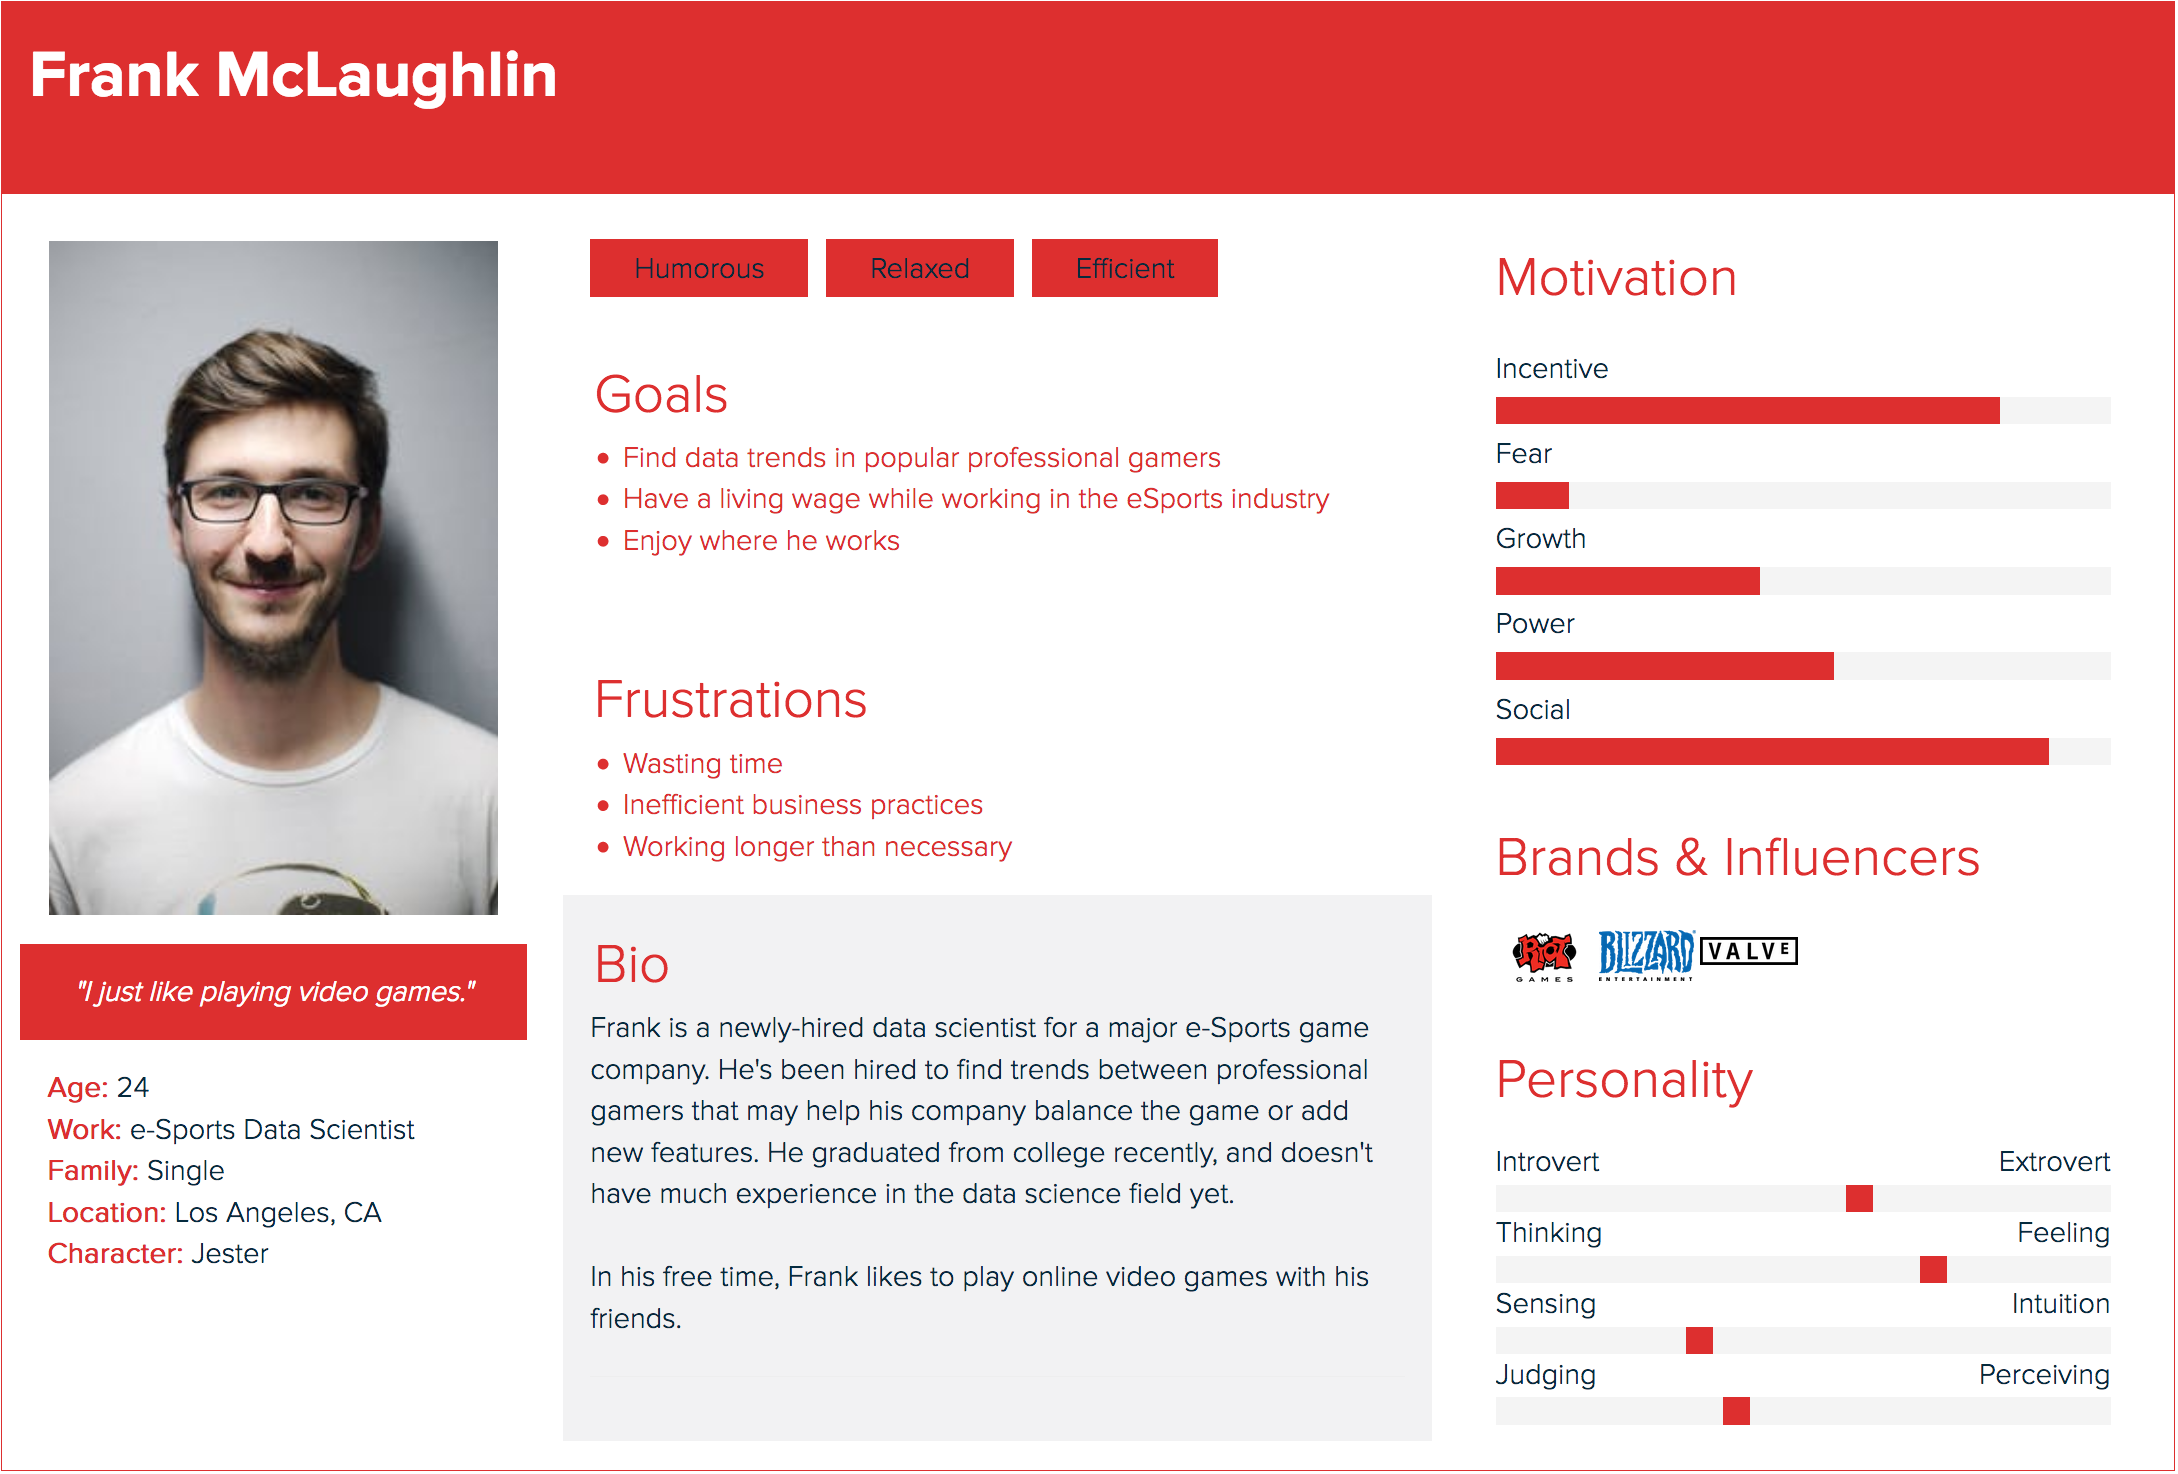
\includegraphics[width = \textwidth]{Frank.png}

\subsection{User Classes and Characteristics}
Identify the various user classes that you anticipate will use this product. User classes may be differentiated based on frequency of use, subset of product functions used, technical expertise, security or privilege levels, educational level, or experience. Describe the pertinent characteristics of each user class. Certain requirements may pertain only to certain user classes. Distinguish the favored user classes from those who are less important to satisfy.  You might use a table like this:
\begin{longtable}{|l|p{3.8in}|}
\hline
\textbf{User Class}&\textbf{Description}\\
\hline
Employee&This is a description of an employee\\
\hline
Administrator&This is a description of an administrator\\
\hline
\end{longtable}

\subsection{Operating Environment}
Describe the environment in which the software will operate, including the hardware platform, operating system and versions, and any other software components or applications with which it must peacefully coexist.
\subsection{Design and Implementation Constraints}
Describe any items or issues that will limit the options available to the developers. These might include: corporate or regulatory policies; hardware limitations (timing requirements, memory requirements); interfaces to other applications; specific technologies, tools, and databases to be used; parallel operations; language requirements; communications protocols; security considerations; design conventions or programming standards (for example, if the customer's organization will be responsible for maintaining the delivered software).
\subsection{User Documentation}
List the user documentation components (such as user manuals, on-line help, and tutorials) that will be delivered along with the software. Identify any known user documentation delivery formats or standards.
\subsection{Assumptions and Dependencies}
List any assumed factors (as opposed to known facts) that could affect the requirements stated in the SRS. These could include third-party or commercial components that you plan to use, issues around the development or operating environment, or constraints. The project could be affected if these assumptions are incorrect, are not shared, or change. Also identify any dependencies the project has on external factors, such as software components that you intend to reuse from another project, unless they are already documented elsewhere (for example, in the vision and scope document or the project plan).
\subsection{Business Rules}
List any business rules.  Identify each one uniquely.


\section{Use Cases}

\subsection{\label{Selecting the Proper Classification from the UIl}Use Case 1: Select Proper Classification Category}
This use case details the the path of the data analyst providing feedback to the machine learning algorithm written by Matt Yarmolich

\begin{longtable}{|r|p{3.8in}|}
\hline
Use Case ID:&1\\
\hline
Use Case Name:&Select Proper Classification Category\\
\hline
Created By:&Matt Yarmolich\\
\hline
Last Updated By:&Matt Yarmolich\\
\hline
Date Created:&October 9, 2018\\
\hline
Date Last Updated:&October 9, 2018\\
\hline
Actors:&Data Analyst\\
\hline
Description:&A Data Analyst accesses the data classification front end by feeding it information from an HTML-5 input tag and having the information parsed by the system. .\\
\hline
Preconditions:&
\begin{packed_enumerate}
\item the Data Analyst is logged into the system.
\item the Data Analyst is a registered user for the system.
\item the Data Analyst has a dataset that needs to be analyzed.
\end{packed_enumerate}\\
\hline
Postconditions:&
\begin{packed_enumerate}
\item the dataset has been correctly parsed by the data classifier
\item the classifier has outputted a variety of tags for verification by the Data Analyst. 
\item the Data Analyst is capable of correctly identifying the dataset
\end{packed_enumerate}\\
\hline
Normal Flow:&1.0 Select the correct category from the data classifier\\
&  %line needed for aligning enumeration 
\begin{packed_enumerate}
\item The Data Analyst uploads the dataset to the front end of the system
\item System displays upload status
\item System displays upload complete and feeds the data to the backend
\item The backend classifies the initial column data
\item The backend classifies the rest of the data based on past data columns and previous data fed through the system
\item the backend outputs the results of the data in a web-parsable format (JSON)
\item The front end parses this output and displays it to the data analyst along with the columns in question
\item the Data Analyst reviews the data and selects the correct category based on their domain knowledge
\item The front end feeds their result back to the data classification backend
\item System displays the correct tagging of the data set
\end{packed_enumerate}\\
\hline
Alternative Flows:&1.1 No results from backend (branch after step )\\
&  %line needed for aligning enumeration 
\begin{packed_enumerate}
\item The system outputs no previously learned categories
\item The Data Analyst inputs a new category for the data set
\item Return to step 8.
\end{packed_enumerate}\\
\hline
Exceptions:&1.0.E.1 System loses connection to front end(at step 1)\\
&1. 	System informs Data Analyst that connection has been lost to the server\\
&2.	Patron reloads page\\
&3.	System restarts use case.\\
\hline
Includes:&None\\
\hline
Priority:&High\\
\hline
Frequency of Use:&Approximately n uses per data set (depends on column inputted)\\
\hline
Business Rules:&TBD\\
\hline
Special Requirements:&
\begin{packed_enumerate}
\item Patron shall be able to cancel the meal order at any time prior to confirming the order.
\item Patron shall be able to view all meals he ordered within the previous six months and repeat one of those meals as the new order, provided that all food items are available on the menu for the requested delivery date. (Priority = medium)
\end{packed_enumerate}\\
\hline
Assumptions:&Assume that 30 percent of Patrons will order the daily special (source: previous six months of cafeteria data).\\
\hline
Notes and Issues:&
\begin{packed_enumerate}
\item The default date is the current date if the Patron is using the system before today's order cutoff time. Otherwise, the default date is the next day that the cafeteria is open.
\item If Patron doesn't want to have the meal delivered, the precondition requiring registration for payroll deduction is not applicable.
\item Peak usage load for this use case is between 8:00am and 10:00am local time.
\end{packed_enumerate}\\
\hline
\end{longtable}


\subsection{\label{Upload Data Sets}Use Case 2: Upload Data Sets}
This use case details the the user flow of uploading data sets to the data classifier using the web interface, written by Spencer Schurk.

\begin{longtable}{|r|p{3.8in}|}
\hline
Use Case ID:&2\\
\hline
Use Case Name:&Upload Data Sets\\
\hline
Created By:&Spencer Schurk\\
\hline
Last Upadted By:&Spencer Schurk\\
\hline
Date Created:&October 10, 2018\\
\hline
Date Last Updated:&October 10, 2018\\
\hline
Actors:&Data Analyst\\
\hline
Description:&After logging in, the system allows a data analyst to upload multiple data sets. After uploading data sets, the data analyst can begin the classification process.\\
\hline
Preconditions:&\begin{packed_enumerate}
\item The data analyst is logged into the system.
\item The data analyst has not uploaded any data sets.
\item The data analyst has not began the classification process.
\end{packed_enumerate}\\
\hline
Postconditions:&\begin{packed_enumerate}
\item All selected data sets have been uploaded.
\item The data analyst is now able to begin the classification process.
\end{packed_enumerate}\\
\hline
Normal Flow:&1.0 Select multiple files to upload.\newline
\begin{packed_enumerate}
\item The data analyst selects "Upload Files" button.
\item System opens local machine's file explorer / file selector.
\item Data analyst selects multiple files from their local machine.
\item Data analyst selects "Ok" or "Upload" on system file explorer.
\item System displays list of files selected and begins to upload files.
\item System displays progress of each file being uploaded.
\item System displays "Upload successful" message after upload completes.
\item Data analyst selects "Begin Classification" button.
\end{packed_enumerate}\\
\hline
Alternate Flows:&1.1 Select files more than once. (branch after step 4)\newline
\begin{packed_enumerate}
\item While previously selected files are uploading, data analyst selects "Upload more files"
\item System opens local machine's file explorer / file selector.
\item Data analyst selects multiple files from their local machine.
\item Data analyst selects "Ok" or "Upload" on system file explorer.
\item System adds selected files to list of previously selected files that are uploading.
\item Flow continues on step 8 of normal flow
\end{packed_enumerate}\\
\hline
Exceptions:&1.0.E.1 Data analyst uploads unsupported file. (at step 4)\newline
\begin{packed_enumerate}
\item System displays error message, with file name present.
\item Data analyst selects "OK" button.
\item System removes selected file from list of files to upload.
\item System continues to upload other selected files.\newline
\end{packed_enumerate}
1.0.E.2 Upload fails for any reason. (at step 5)\newline
\begin{packed_enumerate}
\item System displays "Upload failed" message
\item Data analyst selects "Try again" or "Cancel" button.
\item If "Try again" is selected, system continues at step 5, with all progress at 0.
\item If "Cancel" button selected, page is refreshed, and continues at step 1.
\end{packed_enumerate}\\
\hline
Includes:&None\\
\hline
Priority&High\\
\hline
Frequency of Use:&Once per data classification process.\\
\hline
Business Rules:&TBD\\
\hline
Special Requirements:&TBD\\
\hline
Assumptions:&\begin{packed_enumerate}
\item Data sets are locally stored on data analyst's machine.
\item Data analyst has active internet connection capable of uploading files.
\end{packed_enumerate}\\
\hline
Notes and Issues:&\begin{packed_enumerate}
\item What if the data analyst uploads the wrong file?
\end{packed_enumerate}\\
\hline
\end{longtable}



\subsection{\label{Whatever the next one is}Use Case 3: Whatever the next one is}
This is a casual use-case.  Note that there is a label in the LaTeX so you can refer
to it as being in section~\ref{Whatever the next one is} on page~\pageref{Whatever the next one is}.
\begin{enumerate}
\item This is step one.
\item This is step two.
\item This is step three.
\end{enumerate}

\section{System Features}
This system will be primarily used for data classification and adding meta-tags/titles to unidentified datasets inputted by a user from various formats including CSVs, JSON, and SQL. The main purpose of this product is to give Data Scientists, Data Engineers, and Data Analysis's insight on what kind of data they are collecting, and the ability to verify or modify any tags generated by the machine learning processes in our backend. This will be done through a front end written for the web interfacing with most modern browsers with javascript enabled. This front end will be powered by a backend written in Python leveraging a machine learning library such as TensorFlow. This backend will take data in from a recognized data format, parse the data into a data structure for temporary storage, feed it into this library and spit out possible classification tags. These tags will then be sent to the front end for verification by the data analyst for verification/modification. This data analyst will be able to see the data in question in order to judge the classifiers accuracy and to teach it about new datasets/data types by piping these recommendations back to the machine learning algorithm.

  \subsection{Machine Learning Python Backend}
\subsubsection{Description and Priority}
This feature of the product will allow data being fed into the product to produce meaningful data for output/viewing by the data analyst. The benefit of this algorithm is that it will provide data to the front end for easy viewing and provide an endpoint for where feedback from the data analysts. In terms of cost, this is probably going to be a fairly expensive feature to implement as its the main focus of this project and without it, the rest of the project is useless. However there are a ton of resources for implementing this feature minimizing the potential development time required. Finally, this system requirement is of High priority due to the fact it is the main feature that makes our product useful. 
\subsubsection{Stimulus/Response Sequences}
The system shall take in a dataset from the front end and then feed this dataset into the machine learning algorithm column line by line. This step will be done by the data parser which will read in the columns line by line and separate them (detailed below). This data will then be compared to previous inputs taught by the algorithm by the Software Engineers developing the program. With these comparisons, the algorithm shall develop a result that fits the dataset, or output unknown if it doesnt have any idea what the dataset is of. It also will look to previous classifications contained by the dataset 
\subsubsection{Functional Requirements}
Itemize the detailed functional requirements associated with this feature. These are the software capabilities that must be present in order for the user to carry out the services provided by the feature, or to execute the use case. Include how the product should respond to anticipated error conditions or invalid inputs. Requirements should be concise, complete, unambiguous, verifiable, and necessary. Use "TBD" as a placeholder to indicate when necessary information is not yet available.\\
\\
Each requirement should be uniquely identified with a sequence number or a meaningful tag of some kind.

\begin{enumerate}
\item REQ-1: The system shall be able to take in a specific data column and be able to identify it based on previous machine learning techniques used on the system and output a string of what it thinks it should output .
\item REQ-2: The system shall be able to learn new classifications given to it by the Data Analysts as feedback from the front end.
\item REQ-3: The system shall be able to learn categories over time as training is provided to it by the Software Engineers developing the system, and by data analysts feeding it new categories/training.
\end{enumerate}

\subsection{Data Classification Front End}
\subsubsection{Description and Priority}
This feature set will allow the data analyst to interact with the output of the machine learning algorithm for further classification and viewing of what the algorithm outputs. This feature set is another high priority feature as it allows our algorithm to be interacted with by the client and provide meaningful responses to help further teach the algorithm about new datasets and expectations. 
\subsubsection{Stimulus/Response Sequences}
List the sequences of user actions and system responses that stimulate the behavior defined for this feature. These will correspond to the dialog elements associated with use cases.
\subsubsection{Functional Requirements}
\begin{enumerate}
\item REQ-1: WIP
\item REQ-2: WIP
\item REQ-3: WIP
\end{enumerate}

\subsection{Data Parser}
\subsubsection{Description and Priority}
This feature set will allow the data analyst to submit data to the System and parse it into a computer readable interface and parse it into a data structure for storage and analysis. \subsubsection{Stimulus/Response Sequences}
The data analyst will select a data set to upload to the server. The server will then accept this file and parse the file. During parsing, the computer will store each columns data in separate data structures for analysis. 
\subsubsection{Functional Requirements}
\begin{enumerate}
\item REQ-1: The system shall accept data to be uploaded to the backend
\item REQ-2: The system shall parse the data, storing each row's data for each column in a separate dynamically growing
\item REQ-3: The system shall feed the data to the machine learning algorithm
\item REQ-4: The system shall be able to accept over 10 data sets to upload at a time. (Written by Spencer Schurk)
\end{enumerate}

\section{External Interface Requirements}
\subsection{User Interfaces}
Describe the logical characteristics of each interface between the software product and the users. This may include sample screen images, any GUI standards or product family style guides that are to be followed, screen layout constraints, standard buttons and functions (e.g., help) that will appear on every screen, keyboard shortcuts, error message display standards, and so on. Define the software components for which a user interface is needed. Details of the user interface design should be documented in a separate user interface specification.
\subsection{Hardware Interfaces}
Describe the logical and physical characteristics of each interface between the software product and the hardware components of the system. This may include the supported device types, the nature of the data and control interactions between the software and the hardware, and communication protocols to be used.
\subsection{Software Interfaces}
Describe the connections between this product and other specific software components (name and version), including databases, operating systems, tools, libraries, and integrated commercial components. Identify the data items or messages coming into the system and going out and describe the purpose of each. Describe the services needed and the nature of communications. Refer to documents that describe detailed application programming interface protocols. Identify data that will be shared across software components. If the data sharing mechanism must be implemented in a specific way (for example, use of a global data area in a multitasking operating system), specify this as an implementation constraint.
\subsection{Communications Interfaces}
Describe the requirements associated with any communications functions required by this product, including e-mail, web browser, network server communications protocols, electronic forms, and so on. Define any pertinent message formatting. Identify any communication standards that will be used, such as FTP or HTTP. Specify any communication security or encryption issues, data transfer rates, and synchronization mechanisms.

\section{Other Nonfunctional Requirements}
\subsection{Performance Requirements}
The customer has specified that performance is not a concern.
\subsection{Safety Requirements}
During the classification stage, safety is not a concern. After the catalog phase we will begin redacting sensitive information.
\subsection{Security Requirements}
\begin{enumerate}
    \item The software will have two factor authentication and will only allow verified users to access the systems databases.
    \item The system shall not parse any uploaded data set until the user has selected "Begin Classification." (Written by Spencer Schurk)
\end{enumerate}

\subsection{Software Quality Attributes}
\begin{enumerate}
    \item The system shall have a learning curve of 24 hours. This applies to all users ranging from a sports analyst to a data scientist.
    \item The system shall be available 99.99\% of the time.
    \item The system shall be able to maintain one million datasets.
    \item The system will be portable so different companies can use our solution.
\end{enumerate}


\section{Other Requirements}
Define any other requirements not covered elsewhere in the SRS. This might include database requirements, internationalization requirements, legal requirements, reuse objectives for the project, and so on. Add any new sections that are pertinent to the project.

\appendix
\section{Glossary}
Define all the terms necessary to properly interpret the SRS, including acronyms and abbreviations. You may wish to build a separate glossary that spans multiple projects or the entire organization, and just include terms specific to a single project in each SRS.

\section{Analysis Models}
Optionally, include any pertinent analysis models, such as data flow diagrams, class diagrams, state-transition diagrams, or entity-relationship diagrams.

\section{Issues List}
This is a dynamic list of the open requirements issues that remain to be resolved, including TBDs, pending decisions, information that is needed, conflicts awaiting resolution, and the like.
\end{document}
